\section[Robustness]{Robustness of the DTR for subgroups of data}

The mathematical derivation of uncertainty is to complex for this internship.
To gain a sense of how reliable the effect of DTR change is, we compare the 
results of the left and right hemisphere -- the hemisphere from -180 to 0 and 0 to 180 degrees. 

\begin{figure}[ht]
    \centering
    \begin{subfigure}{0.48\textwidth}
        \centering
        \includegraphics[width = \textwidth]{C:/Users/leonh/Desktop/Praktikum_AWI/NordPolLinks/Lon_66_70/Fit/DTRperMonth.png}
    \end{subfigure}%
    \begin{subfigure}{0.48\textwidth}
        \centering
        \includegraphics[width = \textwidth]{C:/Users/leonh/Desktop/Praktikum_AWI/NordPolRechts/Lon_66_70/Fit/DTRperMonth.png}
    
    \end{subfigure}

    \begin{subfigure}{0.48\textwidth}
        \centering
        \includegraphics[width = \textwidth]{C:/Users/leonh/Desktop/Praktikum_AWI/NordPolLinks/Lon_70_75/Fit/DTRperMonth.png}
    \end{subfigure}%
    \begin{subfigure}{0.48\textwidth}
        \centering
        \includegraphics[width = \textwidth]{C:/Users/leonh/Desktop/Praktikum_AWI/NordPolRechts/Lon_70_75/Fit/DTRperMonth.png}
    \end{subfigure}

    \begin{subfigure}{0.48\textwidth}
        \centering
        \includegraphics[width = \textwidth]{C:/Users/leonh/Desktop/Praktikum_AWI/NordPolLinks/Lon_75_80/Fit/DTRperMonth.png}
    \end{subfigure}%
    \begin{subfigure}{0.48\textwidth}
        \centering
        \includegraphics[width = \textwidth]{C:/Users/leonh/Desktop/Praktikum_AWI/NordPolRechts/Lon_75_80/Fit/DTRperMonth.png}
    \end{subfigure}
    
    \begin{subfigure}{0.48\textwidth}
        \centering
        \includegraphics[width = \textwidth]{C:/Users/leonh/Desktop/Praktikum_AWI/NordPolLinks/Lon_80_84/Fit/DTRperMonth.png}
    \end{subfigure}%
    \begin{subfigure}{0.48\textwidth}
        \centering
        \includegraphics[width = \textwidth]{C:/Users/leonh/Desktop/Praktikum_AWI/NordPolRechts/Lon_80_82/Fit/DTRperMonth.png}
    \end{subfigure}

    \caption{Subfigure with Two Columns}
\end{figure}

The data covers the area represented in \cref{fig:datacoverage}.

\begin{figure}[h]
    \centering
    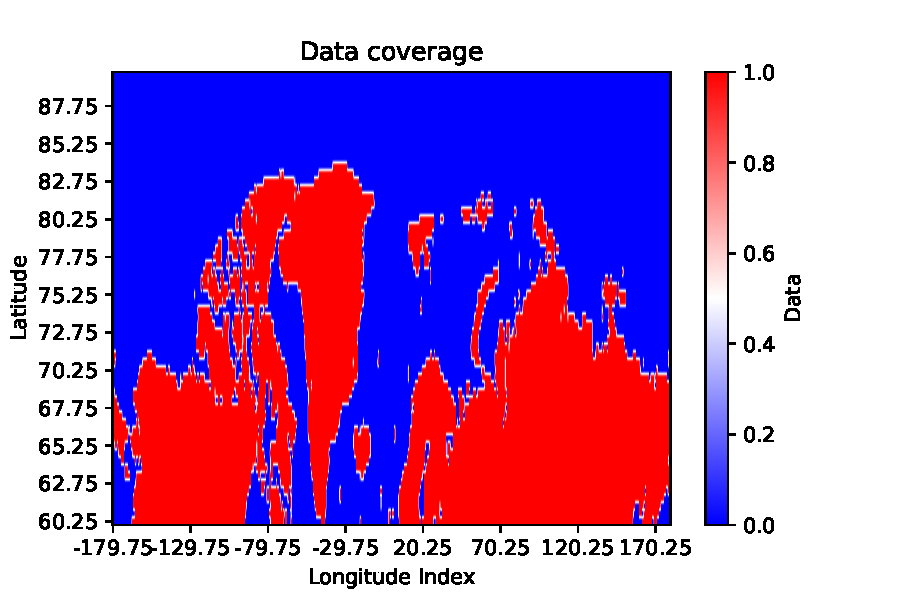
\includegraphics[width = 12cm]{C:/Users/leonh/Desktop/Praktikum_AWI/datacoverage.pdf}
    \caption[short]{Data coverage of the CRU data.}
    \label{fig:datacoverage}
\end{figure}